Конфигурирование модуля \texttt{remap} осуществляется через интерфейс медленного контроля. Как упоминалось ранее, он функционирует поверх протокола Avalon Memory Mapped, который предназначен для работы с адресуемой памятью. Такой подход очень удобен, поскольку в этом случае можно выделить каждому модулю свой участок адресов, по которым можно будет располагать необходимые значения. Разные адреса можно настроить по способу доступа к ним, таким образом можно завести некоторые показатели системы, которые можно будет только считывать, или же добавить параметры с опцией модификации. Отдельная важная особенность работы через память -- возможность функционирования в разных тактовых доменах, для этого достаточно использовать модули двухпортовой памяти. Это позволяет использовать достаточно низкую тактовую частоту для интерфейса конфигурации, чтобы он не оказывал существенного влияния на разводимость остальной логики. Причём эта частота может быть единой для конфигурирования всех компонентов, вне зависимости от их внутренних тактовых сигналов, что значительно упрощает работу медленного контроля.\par
Модуль перестановки \texttt{remap} имеет две конфигурируемые стадии: какие значения извлекать из общего потока данных с помощью мультиплексора и в каком порядке их выдавать в выходной канал. Поскольку эти стадии работают в разных тактовых доменах, то необходимо размещать параметры для них в разных блоках памяти, чтобы можно было корректно переводить значения в целевые тактовые частоты. Начальный адрес конфигурации мультиплексора устанавливается глобальной константой REMAP\_BADDR(Remap Base Address) с уровня всего проекта сигнального процессора LASP, а конфигурация порядка выходных данных имеет некоторое смещение относительно него. На рисунке \ref{fig:remap_sctrl_mapping} изображена схема отображения конфигураций на адресное пространство.\par
\begin{figure}[ht]
    \centering
    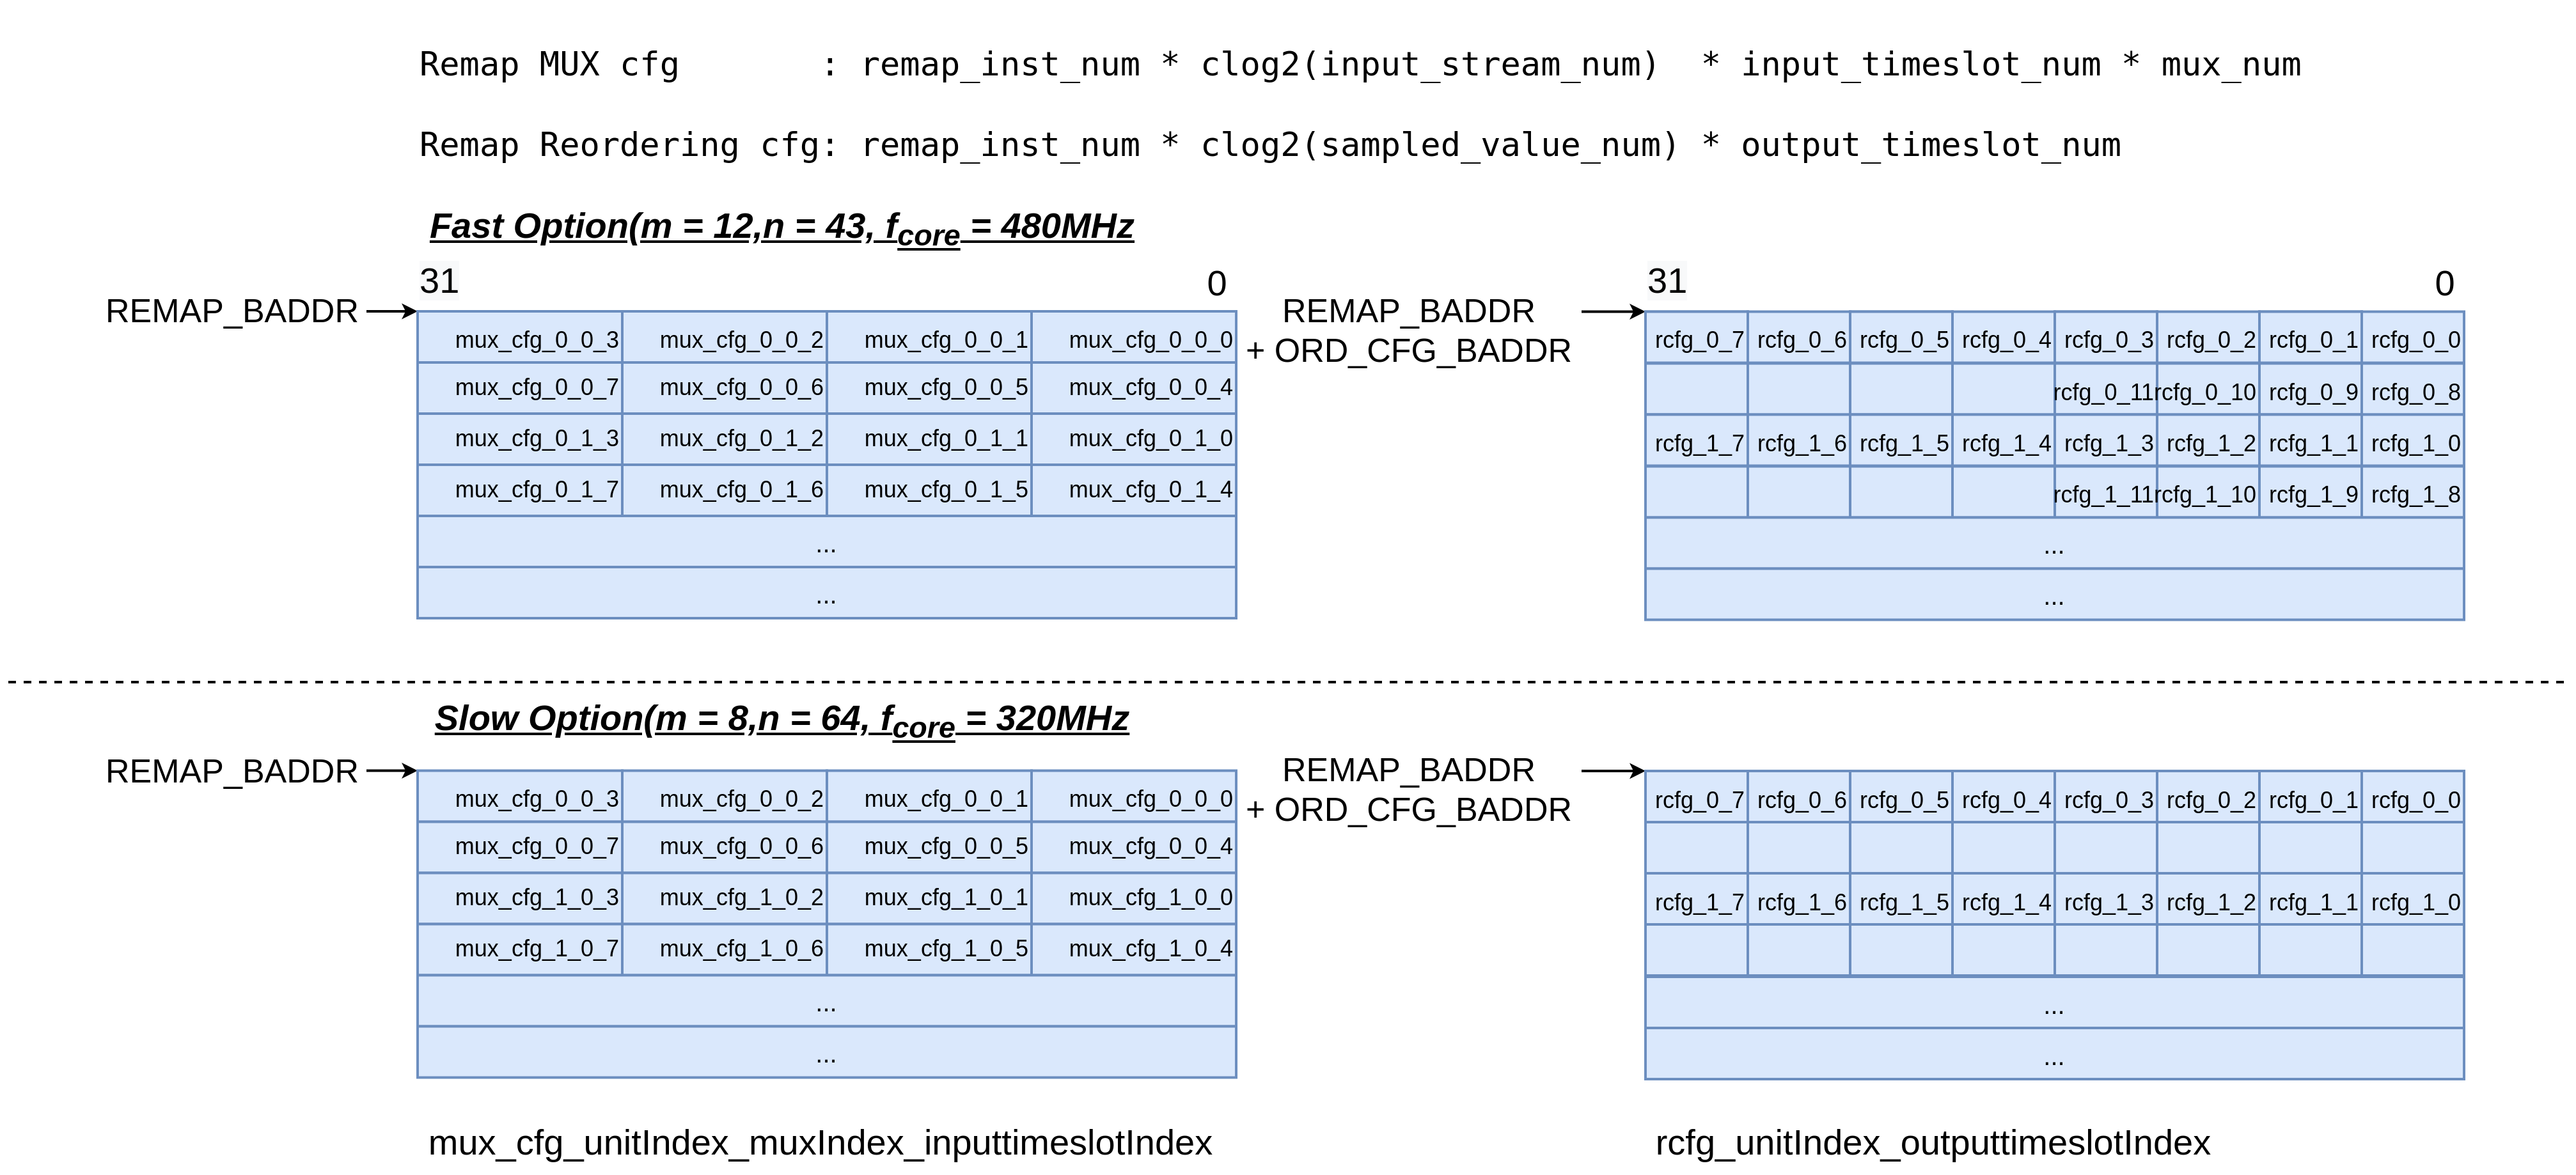
\includegraphics[width=\linewidth]{remap_sctrl_mapping.png}
    \caption{Схема маппинга памяти модуля перестановки \texttt{remap} для записи конфигурации}
    \label{fig:remap_sctrl_mapping}
\end{figure}\par
Для конфирурирования входного мультиплексора необходимо для каждой временной ячейки установить номер канала, с которого необходимо захватить данные. На каждый \texttt{remap} поступает по 22 канала, то есть требуется 5 бит на значение. Для любого столкновения пучков выделяется по 8 временных интервалов, следовательно суммарно должно быть не менее 40 бит данных для конфигурирования одного выходного канала \texttt{remap}. Шина данных интерфейса Avalon Memory Mapped имеет ширину 32 бита, поэтому для удобства формирования и чтения конфигурационных данных используется 2 слова AVMM, что составляет 64 бита. В случае варианта быстрой опции сигнального процессора LASP требуется два входных мультиплексора, соответственно размер конфигурации удваивается и равняется 128 бит.\par
Конфигурирование финальной перестановки осуществляется путём последовательного указания индекса необходимого значения. В зависимости от медленной или быстрой опции отобранных величин может быть 8 или 16 соответственно. Для более удобной работы под каждое такое значение выделяется по 4 бита. Далее, в зависимости от варианта сигнального процессора LASP требуется от 8 до 12 временных ячеек для каждого BCID, следовательно суммарно необходимо иметь от 32 до 48 бит. Аналогично конфигурации мультиплексора, в целях повышения удобства размер конфигурации округляется по ширине шины интерфейса AVMM и составляет 64 бита независимо от опции сигнального процессора LASP.\par
